\chapter{基于随机Top-$k$算法的拆分学习效率优化}
\label{chap:randomized_topk}

拆分学习是一种简单的隐私保护机器学习方法,其适用于纵向联邦学习和隐私推断的场景。
%
在拆分学习中,各方交换模型的中间表征或梯度,实现多方的推断和训练。
%
尽管拆分学习的效率远高于基于密码学的隐私保护机器学习方法,但是其效率依然存在进一步优化的空间。
%
本章探索了拆分学习通信效率的优化方法,对稀疏、量化、缩小拆分层等方法进行了研究,从收敛和泛化两个角度进行优化,最终提出随机top-$k$稀疏化方法,提高了拆分学习的通信效率。
%

\section{研究背景}
随着社会的数据隐私保护意识的提升和相关法律法规的出台,许多隐私保护机器学习方法被提出。
%
拆分学习~\cite{vepakomma2018split,poirot2019split}作为纵向联邦学习~\cite{liu2024vertical}的一种主要方法,有着效率较高、实现简单的优势,因此获得了工业界和学术界的广泛关注~\cite{palanisamy2021spliteasy,koda2020split_mmwave,fagbohungbe2022split_edge_image,roth2022split_unet}。
%


\begin{figure}[htbp]
    \centering
    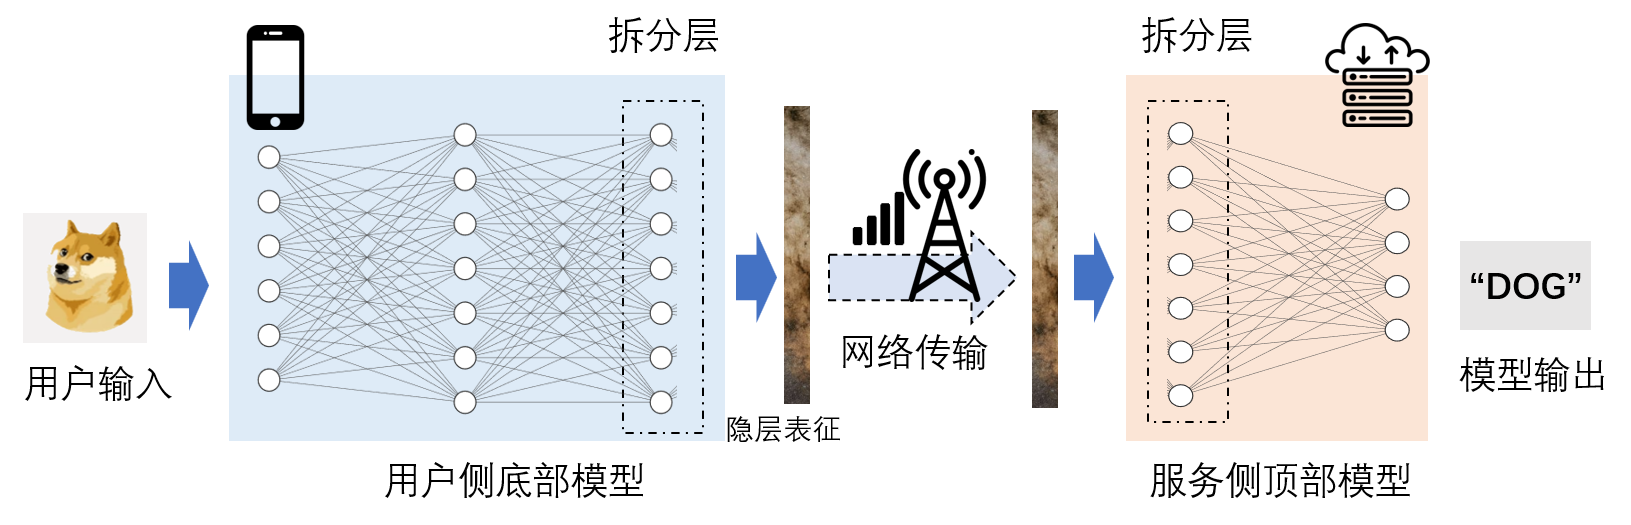
\includegraphics[width=\linewidth]{Z_Resources/随机topk_两方拆分学习示意图.png}
    \caption{两方拆分学习推断示意图}
    \label{fig:randomized_topk-split_example}
\end{figure}

拆分学习的思想是把模型拆分成多个部分分发给各个参与方,各方以交换中间结果的方式进行模型训练和推断,从而实现一定程度上的隐私保护。
%
\autoref{fig:randomized_topk-split_example}显示了一个典型的两方拆分学习的推断场景,我们假设用户具有输入数据,而服务器拥有一个分类模型。
%
进行拆分学习的推断时,用户拥有底部模型,而服务器拥有顶部模型。用户将输入输入底部模型获得隐层表征后,通过网络传输给服务器,然后将其输入顶部模型,从而得到最终的模型预测值。
%
在此过程中,用户只暴露了输入数据的隐层表征,因此其原始输入获得了一定的保护;而服务器只暴露了底部模型而非完整模型,因此模型的隐私也在一定程度上得到了保护。
%
虽然拆分学习的效率相对于密码学方法很高,但是由于拆分学习训练过程中依然需要在每一轮传输隐层特征和梯度,考虑到许多深度学习模型的隐层空间较大,因此拆分学习在通讯效率上依然存在可以优化的空间。
%



本文主要关注类别数量多的深度学习模型场景。
%
分类模型往往可以拆分为特征抽取器和分类器两个部分,其中,特征抽取器的结构较为复杂,可以包含卷积层、长短期记忆层等;而分类器可能是一层简单的全连接层。
%
但是在类别数量众多的情况下,分类器往往包含了模型的大部分参数,如:
%
推荐系统模型~\cite{jannach2017gru4rec,kang2018sasrec}的最后一层可能包含了所有商品的嵌入向量(Embedding Vector);
%
人脸识别模型~\cite{parkhi2015deepface}的最后一层可能包含了所有用户的人脸对应的嵌入向量。
%
在这种情况下,若简单地将整个模型部署到用户侧,既会占用大量的用户侧存储空间,也会带来模型隐私泄露的风险。
%
因此,在这种情况下,就需要采用拆分学习的方式来提高效率,同时保护用户输入和模型参数的隐私。

当前关于纵向联邦学习通讯压缩的研究相对较少,仅有对基础压缩算法的收敛性分析~\cite{castiglia2022compressed_vfl}、拆分层嵌入自编码器~\cite{ayad202vfl}等,前者仅考虑了基本的压缩方法且只应用于训练阶段,而后者只针对拆分学习的一个特定场景。
%
关于提升横向联邦学习的通讯效率的工作则较多,包括了加快收敛速度~\cite{karimireddy2020scaffold,reddi2020fed_opt}、压缩每一轮传输的梯度值~\cite{wen2017terngrad,aji2017sparse,sattler2019sparse_binary}等。
%
前者并不适用于拆分学习,因此本文主要研究如何压缩拆分学习训练和推断过程中传递的中间结果或中间梯度信息。
%


\section{压缩方法初步研究}
本节介绍了几种基础的可以对拆分学习的通信量进行压缩的方法,包括缩小拆分层、Top-$k$稀疏、量化拆分层、使用L1损失函数诱导稀疏,并对各方法进行初步分析。
%
在以下的分析中,我们将拆分学习的底部模型记作$M_b$,顶部模型记作$M_t$,输入、中间结果、输出分别记作$X, H, Y$。
我们使用$d$表示初始的拆分层的维度,$k$表示拆分层压缩后的维度。


\textbf{缩小拆分层}:
在拆分学习中,每一轮训练或推断都会传输拆分层(Cut Layer)的表征以及(训练时)梯度。
%
因此,缩小拆分层的大小可以直接减少拆分学习每一轮的通信量。
%
假设1个全连接网络的隐层维度分别是1000(输入)-100(第1层)-100(第2层/拆分层)-10(输出层),则每一轮前向传播需要传输100个数值;若把拆分层维度缩小到10,则只需要传输10个数值。
%
同样地,在反向传播过程中,也只需要传输10个梯度值。
%
因此,这种方法可以削减90\%的每轮通信量。

\textbf{量化拆分层}:
量化指的是将较高比特位的值(如32位浮点数)转化为较小比特位的近似值(如16位浮点数,4位整数,甚至1位的0/1布尔值)~\cite{zhou2016dorefa,banner2018_8bit,yang2019quantization}。
%
其在神经网络中被广泛应用于减少计算和存储开销。
%
通过对拆分层的值以及梯度进行量化压缩,也可以减少拆分学习训练和推断过程中的通信量。
%
本文考虑最常用的等距均匀量化(Uniform Quantization),对于一个隐层向量$\bvec{h} = (h_1, \cdots, h_d)$,将其量化为 $b$ 比特的量化方法为:
\begin{equation}
    \bvec{h}^C = \mathsf{Compress}(\bvec{h}) = \left( \left\lfloor \dfrac{h_1 - h_\text{min}}{h_\text{max} - h_\text{min}} \cdot  2^b \right\rfloor, \cdots, \left\lfloor \dfrac{h_n - h_\text{min}}{h_\text{max} - h_\text{min}} \cdot 2^b \right\rfloor \right),
\end{equation}
其中,$h_\text{min}$ 和 $h_\text{max}$ 分别表示向量$\bvec{h}$中的最小值和最大值。
%
而解压缩的过程则可以表示为:
\begin{equation}
    \bvec{h}' = \mathsf{Decompress}(\bvec{h}^C) = \left(\cdots, h_\text{min} + \big(h^C_i + \dfrac12 \big) \big(\dfrac{h_\text{max} - h_\text{min}}{2^b}\big), \cdots \right).
\end{equation}
% 
尽管量化压缩可以应用于前向传播的隐层值和反向传播的梯度值,但是在实验中我们发现,如果将量化压缩同时应用于前向传播和反向传播,会带来严重的模型效果损失。
%
考虑到本文主要关注拆分学习推断过程中的通信压缩,因此只将量化压缩应用于反向传播的隐层梯度中。

\textbf{Top-$k$稀疏化}:
Top-$k$稀疏化指在向量中只保留$k$个绝对值最大的元素,而将其他元素置为0。
%
在这种情况下,只需要传输$k$个元素的值和下标。
%
如果在前向传播中应用了Top-$k$稀疏化,则较小的$d-k$个元素没有参与顶部模型的计算,因此在反向传播过程中也无需传播这$d-k$个元素的信息。
%
Top-$k$稀疏化可以自然地同时应用于前向传播和反向传播~\cite{jayakumar_2020_topkast}。
%

\textbf{L1正则化}:L1正则化通过L1损失来诱导稀疏性,被广泛应用在不同的机器学习领域~\cite{tibshirani1996lasso,wright2008sparse_face,yin2012kernel,hoefler2021sparse_deeplearning}。
%
具体来说,在拆分学习的训练过程中,我们在原有的损失函数上加入一个对于拆分层表征向量的L1损失:$L' = L + \lambda \sum_{i=1}^d |h_i|$。
%
其中,$\lambda$用于控制稀疏化的强度,越大的$\lambda$会导致越高的稀疏性,但是同时也会降低模型训练的效果。
%
由于L1正则化需要在训练过程中逐渐实现稀疏化,因此其稀疏化只适用于模型的推断阶段,此时我们可以将拆分层表征中接近0的元素删除,类似Top-$k$稀疏化来传播绝对值较大的值和对应的下标。
%


我们将各种方法对应的压缩比率(压缩后大小/压缩前大小)总结在表 \ref{tab:randomized_top-k:compression_ratio}中。
%
对于Top-$k$即L1稀疏化,我们未考虑对下标进行压缩。
%
表中 $N$ 表示初始值的比特位数,一般为32,$k$表示保留的元素的个数。

\begin{table}[h]
    \centering
    \begin{tabular}{ccc}
    \toprule
    \multirow{2}{*}{压缩方法} & \multicolumn{2}{c}{压缩比率} \\ 
    \cmidrule(lr){2-3}
            & 前向传播 & 反向传播 \\ \midrule
    拆分层缩小     & $k/d$       & $k/d$ \\
    $b$比特量化    & $b/N$    & 1 \\
    Top-$k$稀疏化  & $k/d\cdot (1 + \lceil \log_2 d \rceil/N)$ & $k/d$ \\
    L1正则化       & $k/d\cdot (1 + \lceil \log_2 d \rceil/N)$ & 1 \\
    \bottomrule
    \end{tabular}
    \caption{不同压缩方法的压缩比率}
    \label{tab:randomized_top-k:compression_ratio}
\end{table}
\section{随机Top-$k$算法}
\label{sec:randomized_topk:method}
本章节将提出随机Top-$k$算法,其优势来自于两个方面:
(1)从模型泛化(Generalization)角度,Top-$k$稀疏化优于缩小拆分层,因为同等压缩比率下,Top-$k$稀疏化能够提供更大的表征空间和决策边界大小。
(2)从模型训练和收敛的角度,Top-$k$稀疏化会导致部分神经元训练困难,导致收敛变慢,并且无法完全利用表征空间,从而降低其泛化性能上的优势。
%
基于以上两个观察,我们通过在Top-$k$稀疏化中加入随机扰动的方式,解决了第二点的部分神经元训练困难问题,从而提高了模型的收敛速度和泛化效果。
%
下文将对其进行具体的分析。

\subsection{Top-$k$稀疏化和缩小拆分层算法的分析}
首先,我们注意到在输出类别数较多的分类模型中,如果缩小拆分层的神经元数目,模型将会产生更大的泛化误差。
而Top-$k$稀疏化因为在同等压缩率下有更大的样本空间,在理论上可以解决这个问题。


\textbf{增大类间距离可以提高模型泛化性能}:
许多神经网络泛化的研究都表明泛化误差与模型的光滑度(Smoothness)密切相关。
%
简单而言,模型越光滑,其泛化效果越好~\cite{neysharbur2015norm_capacity,neysharbur2017generalization,gouk2021lipschitz_reg}。
%
考虑拆分层在最后一层,激活函数是Softmax的情况。
此时模型的输出值可以写成:
\begin{equation}
    \bvec{y} = \text{Softmax}(\bvec{h}\cdot \bvec{w}_1, \cdots, \bvec{h} \cdot \bvec{w}_n),
\end{equation}
其中,$\bvec{h}$表示拆分层的隐层表征,$\bvec{w}_i$ 表示最后一层权重矩阵的第$i$行,$n$是类别个数。
%
当模型训练到一个较高准确率后,假设$\bvec{h}$对应某个第$i$类样本的拆分层表征,则$\bvec{h}$和$\bvec{w}_i$会比较接近,而和其他的权重$\bvec{w}_{j\ne i}$距离较远。
%
令最短类间距离(Inter-Class Distance)$d_W = \min_{i\ne j} \Vert \bvec{w}_i - \bvec{w}_j \Vert$,
则我们可以估算顶部模型的光滑度为$\Vert \nabla_{\bvec{h}} M_t(\bvec{h}) \Vert \approx c/d_W$,其中$M_t$表示顶部模型,$c$是某个常数。
%
直接理解,$d_W$是两个不同类别对应的权重的最短距离。
当拆分层表征从一个类别的表征$\bvec{w}_i$变化到另一个类别的表征$\bvec{w}_j$时,其最短的移动距离为$d_W$,而模型的输出也应该从$\mathsf{onehot}(i)$变化到$\mathsf{onehot}(j)$。
%
可以看出,$d_W$越小,要实现准确的分类效果,模型的输出就需要变化得越剧烈,也就是模型更不光滑;反之,模型的输出变化可以更加缓慢,模型可以更加光滑。
%
由于光滑性和泛化误差是直接相关的,因此,我们可以使用$d_W$作为一个模型泛化的指标。
%


\textbf{同等压缩率下,Top-$k$稀疏化比缩小拆分层有更大的类间距离}:
首先注意到,类间距离和表征空间(Feature Space)的体积呈正相关---表征空间越大,则可以有更大的类间距离。
%
但是一般神经网络的隐层表征的值域是无限大的,即$\mathbb R^d$,导致最短类间距离无法计算。
%
但是注意到,对于Softmax的多分类层,其分类结果仅仅和隐层表征的方向有关,而和其大小无关。
%
因此,我们可以给拆分层表征空间加上一个范数约束,即$\Vert \bvec{h} \Vert = 1$,而不影响模型输出结果。
%
此时整个表征空间可以划分为$n$个类别的决策区域(Decision Region)。
假设第$i$个类别与其他所有类别的最短类间距离$d_i$和该类别的决策区域大小$s_i$呈现单调递增关系,则很显然得到最短类间距离最大时,各个类别应该有相同的决策区域大小,因为:
\begin{equation}
    \min (s_1, \cdots, s_n), \quad \text{s.t. } {\sum_{i=1}^n s_i = S, s_i > 0}.
\end{equation}
在$s_1 = \cdots = s_n$时取得最小值 $S/n$。
其中,$S$表示表征空间的总面积。

假设表征空间维度为$k$,考虑到$\Vert \bvec{h} \Vert^2 = 1$的约束,则表征空间构成一个$k-1$维超球面,其面积为:
\begin{equation}
    S = 2\pi^{k/2}/\Gamma(k/2).
\end{equation}



我们可以假设样本的决策区域面积约为对应的权重向量的附近的$k-1$维圆形区域面积。
该圆形落在$k-1$维的球面空间,但是在类别数量多的情况下各个类别的决策区域较小,因此可以近似为欧氏空间,此时决策区域的大小可以用圆面积近似表示:
\begin{equation}
    s_i \approx \dfrac{\pi^{(k-1)/2}}{\Gamma((k+1)/2)} \cdot r_i^{k-1},
\end{equation}
其中,$r_i = d_i/2$表示决策区域的半径。
%
%ci
此时,我们可以分别计算缩小拆分层和Top-$k$稀疏化后的类间距离。



\begin{itemize}
    \item 
    缩小拆分层:假设缩小后的拆分层维度为$k$,则表征空间大小为$k$维球体的表面积大小$S = 2\pi^{k/2}/\Gamma(k/2)$。
    而单个类别对应的决策区域为$k - 1$维半径为$r$的圆形,其面积为 $r^{k-1}\pi^{(k-1)/2} / \Gamma[(k + 1)/2]$。
    %
    考虑到总共有$n$个类别,可以得到以下关系:
    \begin{equation}
        n r^{k-1} \cdot \pi^{(k-1)/2} / \Gamma[(k + 1)/2] \approx 2\pi^{k/2}/\Gamma(k/2).
    \end{equation}
    于是可以求出决策边界半径大小:
    \begin{equation}
        r^{k-1} \approx \dfrac{2\sqrt\pi}{n} \cdot \dfrac{\Gamma[(k+1)/2]}{\Gamma[k/2]}.
    \end{equation}
    注意到伽马函数(Gamma Function)的特性 $\Gamma(x + 1/2) \approx \Gamma(x)\times x^{1/2}$,上式可以进一步化简为
    \begin{equation}
        r \approx \left(\dfrac{2}{n} \sqrt{\dfrac{k\pi}{2}} \right)^{1/(k-1)}.
    \end{equation}

    \item
    Top-$k$稀疏化:假设缩小后的拆分层维度为$k'$(在同等压缩率下,$k' < k$,因为需要传输额外的下标信息 )。
    %
    注意到此时的表征空间由${d \choose k'}$ 个$k$维球面组成,因为Top-$k$稀疏化每次从$d$维中选出$k'$维保留。
    %
    因此,类似缩小拆分层的推导,可以得到决策区域半径为:
    \begin{equation}
        r' \approx {d \choose k'} \left(\dfrac{2}{n} \sqrt{\dfrac{k'\pi}{2}} \right)^{1/(k'-1)}.
    \end{equation}
\end{itemize}
%
对两个决策区域半径相除,得到:
\begin{equation}
\label{eq:randomized_topk_r_ratio}
    \dfrac{r'}{r} = \dfrac{d'_W}{d_W} \approx \tilde c := {d \choose k'} \left( \dfrac2n \sqrt{\dfrac{k\pi}{2}} \right)^
    {1/(k'-1) - 1/(k-1)} \sqrt{\dfrac{k'}{k}}^{1/(k' - 1)}.
\end{equation}
%
其中,我们用$\tilde c$表示估计的决策区域半径(类间距离的一半)比值。
%
现在我们考察$k'$和$k$的关系。很显然注意到,神经网络的隐层大小一般不超过$2^{16}\approx 250K$,因此我们最多只需要16个比特来表示每个元素的下标;同时考虑一般的浮点数本身也是32位的,
要约束Top-$k$的压缩率不高于缩小拆分层,只需要满足
$k' +  k'/2 \le k$,其中$k'$表示$k'$个元素的值自身需要$k'$个浮点数的空间,而$k'/2$表示$k'$个下标需要$k'/2$个浮点数的空间(因为16位比特足以表示下标)。
%
因此,可以取$k' = 2/3 k$使得式\eqref{eq:randomized_topk_r_ratio}最大。
%

考虑指数项:
\begin{equation}
    f(k) = \dfrac{1}{k' - 1} - \dfrac{1}{k} = \dfrac{1}{2/3 \cdot k - 1} - \dfrac{1}{k - 1} \le 1/2.
\end{equation}
%
对$k$求导得到:
\begin{equation}
    f'(k) = \dfrac{1}{(k - 1)^2} - \dfrac{1}{(3/2)(2/3 \cdot k - 1)^2}.
\end{equation}
%
注意到在$k \ge 3$时有:
\begin{equation}
    (k - 1)^2 = k^2 - 2k + 1 > 3/2 \cdot (2/3\cdot k - 1)^2 = 2/3 \cdot k^2 -2k + 3/2.
\end{equation}
%
于是,$f'(k) \le 0$ 对$k \ge 3$都成立,同理得到$k \ge 3$时,$f(3) = 1/2 \ge f(k)$。
%



假设$\sqrt{2k\pi} < n$,则$2/n \sqrt{k\pi/2} \in (0, 1)$,又考虑到 $a^x$ 在$a \in (0, 1)$时单调递减,代入式\eqref{eq:randomized_topk_r_ratio},可以得到:
\begin{equation}
    \tilde c \ge \dfrac23 {d \choose k'} \left(\dfrac{2k\pi}{n^2}\right)^{1/4}.
\end{equation}
%
在${d \choose k'} > \sqrt{n}$ 的情况下,该式大于1。
%
举例来说,比如原始的特征维度$d = 1000$,类别数目$n = 1000$,稀疏化后的$k = 6$, $k' = 4$,则有$\tilde c \approx 10^{10} \gg 1$。
%
若将特征维度缩小到$d = 100$,则$\tilde c \approx 10^6 \gg 1$。
%

通过以上推导可以看出,使用Top-$k$稀疏算法时,虽然保留的维度变少了一些,但是由于引入了${d \choose k'}$这一组合项,使得表征空间远大于同等压缩率下直接缩小拆分层的方法。
%
因此,从理论上来说Top-$k$稀疏化将使模型具有更好的泛化性能。
%


\subsection{Top-$k$算法训练收敛问题}
尽管上文的推导证明Top-$k$稀疏化具有更好的泛化性能,但是其依然可能存在收敛性上的问题。
因为将Top-$k$稀疏化运用在训练过程中时,存在“赢家通吃”的问题,导致非Top-$k$的神经元可能难以得到训练。
%
具体而言,假设一个神经元对应的输入权重都较低,那么这个神经元很可能在不同的输入样本上都会获得较小的激活值,从而导致其一直无法得到训练。
%
在这种情况下,Top-$k$可能陷入局部最优。
%
下文将用一个简单的例子来说明Top-$k$陷入局部最优的情况。

考虑如下的目标函数:
\begin{equation}
    f: (x_1, x_2) \to \text{Sign}(x_1 - x_2),
\end{equation}
以及如下的拆分逻辑回归模型:
\begin{equation}
\begin{cases}
    M_b: & (x_1, x_2) \to (h_1, h_2) = (w_1x_1, w_2x_2), \\
    M_t: & (h_1, h_2)\rightarrow \text{Tanh}(h_1 + h_2).
\end{cases}
\end{equation}
这里我们用$x_1, x_2 \in \mathbb R$表示二维的输入特征,$h_1, h_2 \in \mathbb R$表示拆分层的表征,而$w_1, w_2$表示底部模型的权重,初始值为$w_1 = 1, w_2 = -0.1$。


假设有以下两个训练样本:
\begin{equation}
\begin{cases}
    \bvec{x}_1 = (\phantom{0.}1, \, 0), \quad y_1 = \phantom{-}1, \\
    \bvec{x}_2 = (          0.5, \, 1), \quad y_2 = -1.
\end{cases}
\end{equation}
%
很容易可以看出,在Top-$k$($k=1$)稀疏的情况下,$w_1 \to +\infty, w_2 \to -\infty$ 是最优的权重。
%
我们在\autoref{fig:randomized_topk:example}中显示了这个例子的损失函数曲面和梯度下降方向。


\begin{figure}[htbp]
    \centering
    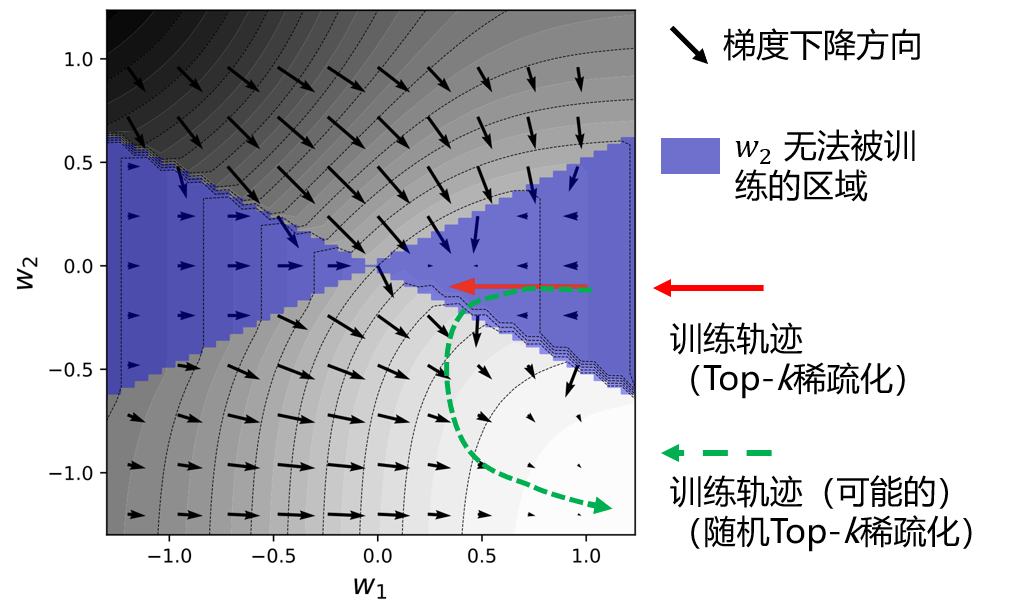
\includegraphics[width=0.75\linewidth]{Z_Resources/randtopk_example.png}
    \caption{使用Top-$k$稀疏化时的损失函数曲面和梯度下降方向}
    \label{fig:randomized_topk:example}
\end{figure}



然而如果在训练过程中使用Top-$k$稀疏化(假设使用平方损失函数),由于$h_2$的值在各个样本上都很小,则$h_2$总是无法被选为Top-$k$,从而导致其对应的权重$w_2$一直无法被训练(对应图中的蓝色区域)。
%
在这种情况下,模型会收敛到一个远离最优点的区域,使得$w_1$降低到$0.4$左右,平衡两个样本的误差,而$w_2$则未被更新而停留在$0.1$处,对应\autoref{fig:randomized_topk:example}中的红色训练轨迹。
%
但是如果在Top-$k$的过程中加入一点随机性,使得$h_2$也有一定的几率被选中,则可以让$w_2$被训练到并且更新,从而摆脱局部最优。
图中的绿色轨迹表明了在Top-$k$稀疏化中加入随机性后产生的一条可能的训练轨迹。


Top-$k$稀疏化的收敛问题也会进一步导致其泛化性能降低。
%
如上文所述,Top-$k$稀疏化带来的泛化优势是因为其表征空间包含了$d \choose k$个超球面,其中$d$是原始的拆分层维度(神经元个数),$k$是稀疏化后保留的维度。
%
但是由于Top-$k$稀疏化带来某些神经元(维度)一直难以得到训练的问题,导致某些神经元在各个样本都无法被选中为Top-$k$,从而导致这些神经元被在模型中无法发挥作用,缩小了表征空间的大小。
%
具体而言,如果采用Top-$k$算法进行训练,假设有$d'$个神经元处于“废弃”状态,则最终得到的表征空间中的超球面数目就会从$d \choose k$减少到$d - d' \choose k$。
%
同样地,如果在Top-$k$稀疏化中加入随机性,将使得各个神经元都有一定的机会被训练,提高表征空间的利用率,从而提高泛化效果。


\subsection{随机Top-$k$算法定义}
基于以上分析,我们可以定义如下的随机Top-$k$算法:
%
选择$k$个要保留的神经元时,每一次选择某个神经元的概率为:
\begin{equation}
\label{eq:randomized_topk:def}
    P(\text{选择该神经元}) = 
    \begin{cases}
        (1 - \alpha) / N_1  & \text{如果该神经元是Top-$k$的,} \\
        \alpha / N_2        & \text{反之.}    
    \end{cases}
\end{equation}
%
其中,$N_1$和$N_2$分别表示当前未被选择的Top-$k$神经元数目和非Top-$k$神经元数目。
%
\autoref{fig:randomized_topk:algo}显示了随机Top-$k$算法的可能执行结果。
%
可以看出,$\alpha$表示选择非Top-$k$神经元的概率。
%
当$\alpha=0$时,随机Top-$k$算法退化为普通的Top-$k$稀疏化;而当$\alpha=1$时,则转变为完全随机的Dropout算法~\cite{srivastava_2014_dropout}。
%
注意到,随机Top-$k$仅仅被应用于模型的训练阶段,在推断阶段,我们依然采用确定性的Top-$k$稀疏化。
%
通过实验,我们发现$\alpha \in [0.05, 0.1]$时模型能取得较好的训练效果。
%
\begin{figure}[h!]
    \centering
    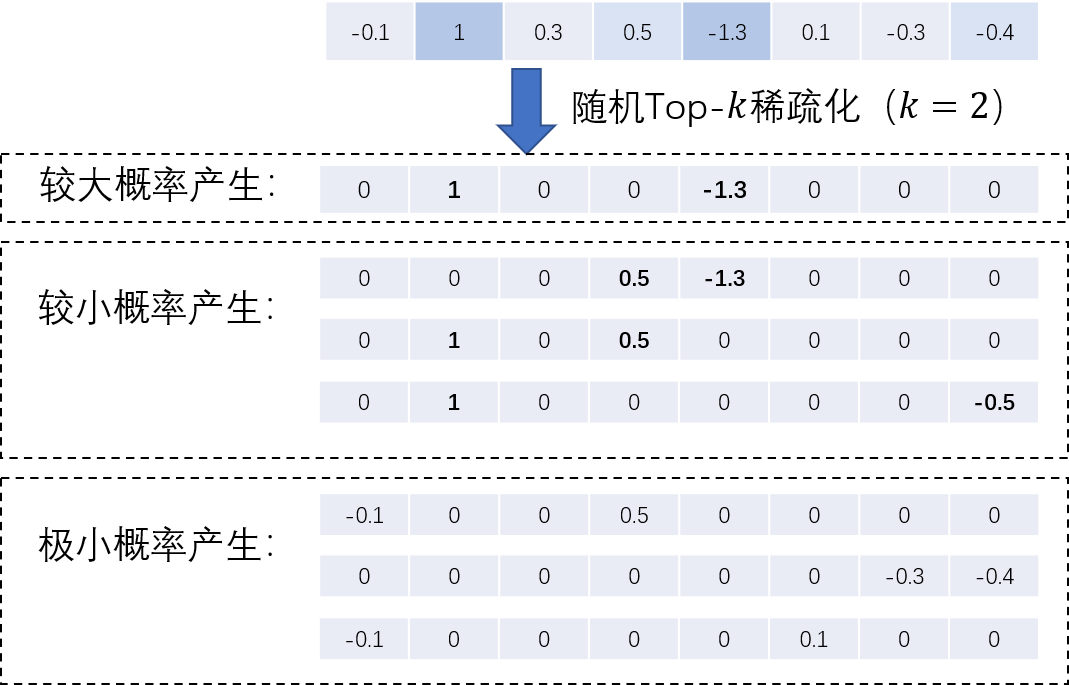
\includegraphics[width=0.7\linewidth]{Z_Resources/randtopk_algorithm.png}
    \caption{随机Top-$k$算法示意图}
    \label{fig:randomized_topk:algo}
\end{figure}


\subsection{隐私分析}
对拆分层表征进行稀疏化后,大部分的拆分层表征元素被丢弃,因此Top-$k$稀疏化或随机Top-$k$稀疏化都能够比原始的拆分学习更多地保护输入特征的隐私。
%
我们在后续实验章节中提供了通过拆分层表征对输入特征进行重建攻击(Reconstruction Attack)的结果。
%
尽管如此,研究表明拆分学习对于标签推理攻击(Label Inference Attack)或模型补全攻击(Model Completion Attack)较为脆弱\cite{fucong2022label_infer_attack},随机Top-$k$算法也并不能解决标签的隐私问题。
%
因此本文考虑的应用场景为标签类别数量大且标签推断攻击不可行的深度学习应用。
%
比如,包含了数千个类别的人脸识别模型、包含了上万种商品的推荐系统模型。
%
对于这些模型,使用者难以获取其他类别对应的输入特征,因此也难以进行标签推断攻击或是模型补全攻击。
%


\section{实验分析}

为了验证本章所提出的随机top-$k$算法的性能,我们在4个不同类型数据集上使用不同的模型进行了实验:
\begin{itemize}
    \item CIFAR-100~\cite{krizhevsky_2009_cifar}: 一个常用的包含了100类总共5万张大小为$32\times 32$的彩色图片。
        我们使用ResNet-20模型~\cite{hekaiming2016resnet}进行分类,拆分层设置为最后的隐层,大小为128。
    %
    \item YooChoose(1/64)~\cite{ben2015yoochoose}:一个推荐系统的数据集,包含了大约15万条用户的点击序列,总共有约1.8万个商品类别。
        我们使用GRU4Rec模型~\cite{jannach2017gru4rec}进行分类,隐层大小设置为300。
        拆分层设置为最后的隐层,大小为300。
    %
    \item DBPedia~\cite{2007dbpedia}:一个文本分类数据集,包含了219种类别,总共有大约34万条文本。
        我们采用TextCNN模型~\cite{kimyoon2014textcnn}进行分类,卷积核的大小为 $(3,4,5)$,并且使用Glove预训练词向量~\cite{pennington2014glove}。
        拆分层设置为最后的隐层,大小为300。
    %
    \item Tiny-Imagenet~\cite{tiny-imagenet}:一个图像分类数据集,包含了200类的10万张彩色图片,图片尺寸为$64\times 64$。
        我们采用EfficientNet-b0模型~\cite{tanmingxing2019efficientnet}进行分类。
        拆分层设置为最后的隐层,大小为1280。
        额外地,我们对权重采用ImageNet的预训练权重和随机初始化两种情况分别进行了实验并汇报结果。
\end{itemize}
%
对于每个任务,我们都测试了不同的模型压缩方法和压缩比率,并且对每一个设定都重复了5次实验取平均值汇报。
%
实验的代码基于Pytorch框架编写,在带有NVIDIA RTX 3090的服务器上进行。
%
实验时我们按照8:1:1的比例划分训练集、验证集合测试集(对于Yoochoose数据集按照先后时间划分),使用Early Stop策略获得验证集上最佳的模型,然后在测试集上进行测试。

\subsection{压缩比率和模型准确率对比}
%
我们测试了模型在测试集上的准确率(对于Yoochoose数据集,我们用前20准确率代替),汇报在。
%
我们把随机top-$k$的随机参数在CIFAR-100, DBPedia, Tiny-Imagenet三个任务上$\alpha$设置为0.1,在Yoochoose任务上设置为0.05。
%
我们把实验结果汇报在\autoref{tab:randomized_topk:main-result}中的。
表内每一项的格式为“准确率/压缩比率*100”,任务名称下方的准确率表示无压缩的普通拆分学习的准确率(压缩比率=100)。
表内空白项表示该方法无法达到对应的压缩比率。
我们用粗体表示同等压缩比率下最高的准确率,用下划线表示次高的准确率。


\begin{table*}[h]
    \centering
    \setlength\tabcolsep{10pt}
    \renewcommand{\arraystretch}{0.8}
    \caption{实验结果:准确率和压缩比率}
    \label{tab:randomized_topk:main-result}
    \small
    \begin{tabular}{@{}ccrrrrr@{}}
    \toprule
    任务          & 压缩  & 随机top-$k$                        & Top-$k$                        & 缩小拆分层             & 量化                 & L1正则化    \\ \midrule
    \multirow{3}{*}{\begin{tabular}[c]{@{}c@{}}CIFAR-100\\      67.20\end{tabular}}\hspace{-3pt}      
        & 高      & \textbf{65.25 / 2.86}       & \underline{62.23 / 2.86} & 55.52 / 3.13       & -                            & -          \\ \cmidrule(lr){2-7} 
        & 中      & \textbf{65.83 / 5.71}       & \underline{61.56 / 5.71} & 60.43 / 6.25       & 53.56 / 6.25          & \underline{62.11 / 8.41}   \\ \cmidrule(lr){2-7} 
        & 低      & \underline{65.98 / 12.4}         & 62.11 / 12.3       & 62.93 / 12.4       & \textbf{66.01 / 12.5} & 63.87 / 19.5          \\ \midrule
    \multirow{3}{*}{\begin{tabular}[c]{@{}c@{}}YooChoose\\      63.57\end{tabular}}\hspace{-3pt}      
        & 高      & \textbf{60.29 / 0.85}       & \underline{60.28 / 0.85} & 50.71 / 1.00       & -                            & -          \\ \cmidrule(lr){2-7} 
        & 中      & \textbf{64.55 / 1.71}       & \underline{63.81 / 1.71} & 62.20 / 2.00       & -                            & -                                   \\ \cmidrule(lr){2-7} 
        & 低      & \textbf{66.88 / 3.84}       & \underline{66.12 / 3.84} & \underline{66.12 / 4.00} & 64.69 / 3.13          & 61.48 / 3.01          \\ \midrule
    \multirow{4}{*}{\begin{tabular}[c]{@{}c@{}}DBPedia\\      93.11\end{tabular}}\hspace{-3pt}        
        & 很高    & \textbf{84.88 / 0.44}       & \underline{83.04 / 0.44} & 64.80 / 0.50       & -                            & -          \\ \cmidrule(lr){2-7} 
        & 高      & \textbf{88.01 / 0.88}       & \underline{85.49 / 0.88} & 78.57 / 1.00       & -                            & 81.35 / 1.08          \\ \cmidrule(lr){2-7} 
        & 中      & \textbf{90.50 / 1.97}       & 87.74 / 1.97       & 86.42 / 2.00       & -                            & \underline{87.88 / 0.93}    \\ \cmidrule(lr){2-7} 
        & 低      & \underline{91.59 / 3.06}          & 90.05 / 3.06       & 88.38 / 3.00       & 91.20 / 6.25          & \textbf{93.11 / 5.31} \\ \midrule
    \multirow{3}{*}{\begin{tabular}[c]{@{}c@{}}Tiny-ImageNet \\ 随机初始化 \\      53.11\end{tabular}}\hspace{-3pt}   
        & 高      & \textbf{50.83 / 0.21}       & 48.36 / 0.21       & 35.46 / 0.23       & -                            & -           \\ \cmidrule(lr){2-7} 
        & 中      & \textbf{51.75 / 0.42}       & \underline{47.24 / 0.42} & 45.66 / 0.47       & -                            &  -                                 \\ \cmidrule(lr){2-7} 
        & 低      & \textbf{51.16 / 0.94}       & 45.50 / 0.94       & \underline{48.87 / 0.14} & -                            & -                                   \\ \midrule
    \multirow{3}{*}{\begin{tabular}[c]{@{}c@{}}Tiny-ImageNet \\ 预训练 \\ 75.18\end{tabular}}\hspace{-3pt} 
        & 高      & \textbf{71.09 / 0.21}       & \underline{70.86 / 0.21} & 59.23 / 0.23       & -                            & -           \\ \cmidrule(lr){2-7} 
        & 中      & \textbf{72.15 / 0.42}       & \underline{71.19 / 0.42} & 66.52 / 0.47       & -                            & -                                   \\ \cmidrule(lr){2-7} 
        & 低      & \textbf{73.83 / 0.94}       & \underline{72.52 / 0.94} & 68.67 / 0.94       & -                            & 67.82 / 1.24          \\ \bottomrule
    \end{tabular}
\end{table*}


实验结果表明,随机top-$k$算法几乎在所有任务上都取得了最好的准确率和最低的压缩比率,且大幅领先于其他方法,在很低的压缩比率情况下依然保持了和原始无压缩拆分学习相近的表现。
%
在YooChoose任务中,随机top-$k$算法甚至超过了无压缩的拆分学习,我们认为这可能归功于随机top-$k$的正则化效果。
%
同时,我们注意到,量化方法和$L1$正则化方法在无法达到一些较低的压缩比率。
这是因为量化方法最低智能达到1/32的压缩比率,并且此时拆分层表征被压缩为2值,往往会导致模型无法收敛。
而$L1$正则化在系数过大时也会导致模型无法收敛。
%

\subsection{训练速度分析}
\begin{figure}[h!]
    \centering
    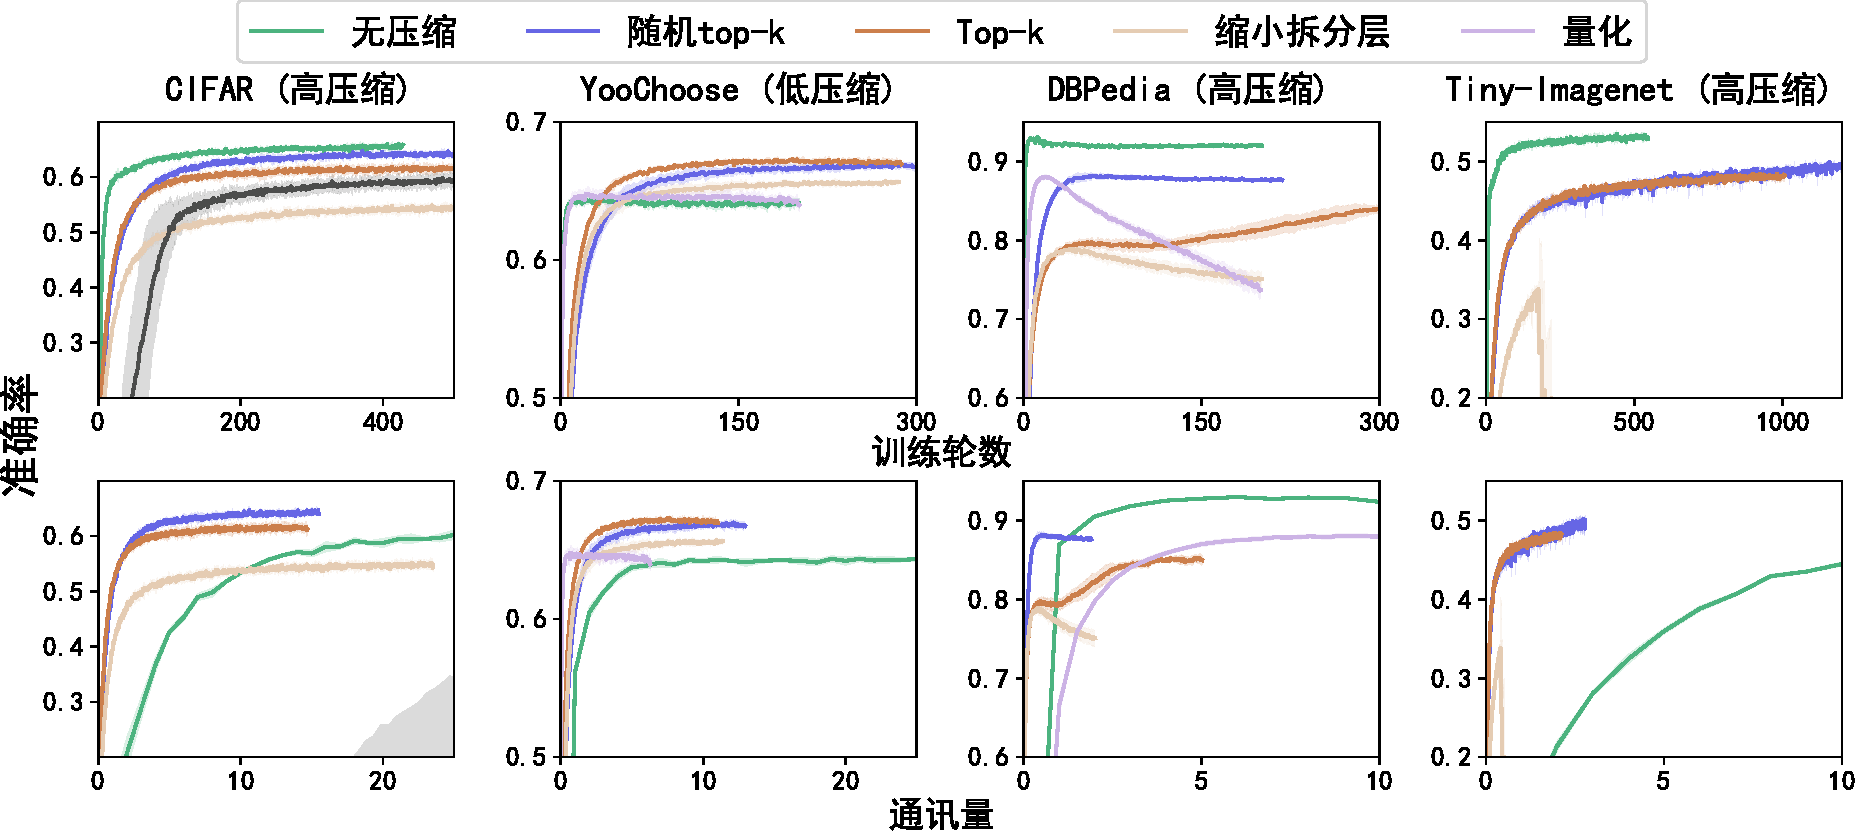
\includegraphics[width=1\linewidth]{Z_Resources/随机topk_训练曲线.pdf}
    \caption{训练轮次/通讯量和准确率}
    \label{fig:randomized_topk:training}
\end{figure}


我们在\autoref*{fig:randomized_topk:training}中汇报了训练过程中准确率和训练轮次以及通信量的关系。
图的第一行是训练轮次和准确率的对比,第二行是通信量和训练轮次的对比,其中我们把一轮无压缩的拆分学习的通信量设为1。
%
实验结果表明,无压缩的拆分学习收敛所需要的训练论次数最少。
但是以通信量衡量时,几乎所有压缩方法的收敛所需的通信量都不无压缩的拆分学习少,并且相比于其他方法,随机top-$k$的收敛速度和准确率都是最高的。
%

\subsection{随机参数$\alpha$分析}
本节我们汇报了变化随机参数$\alpha$时的实验结果,包括了$\alpha$和准确率、收敛速度、泛化误差,top-$k$神经元分布、以及输入特征重构攻击效果的关系,为选取合适的$\alpha$提供参考,并且印证前文关于收敛性、泛化效果以及隐私保护的理论分析。


\begin{figure}[h!]
    \centering
    \begin{subfigure}{0.46\linewidth}
        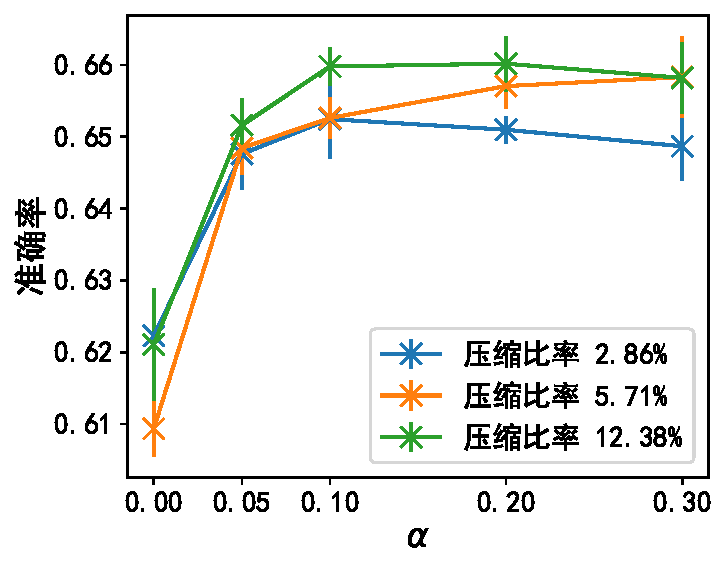
\includegraphics[width=1\linewidth]{Z_Resources/随机topk_cifar-alpha.pdf}
        \subcaption{CIFAR.}
        \label{fig:cifar-trainloss}
    \end{subfigure}
    \begin{subfigure}{0.46\linewidth}
        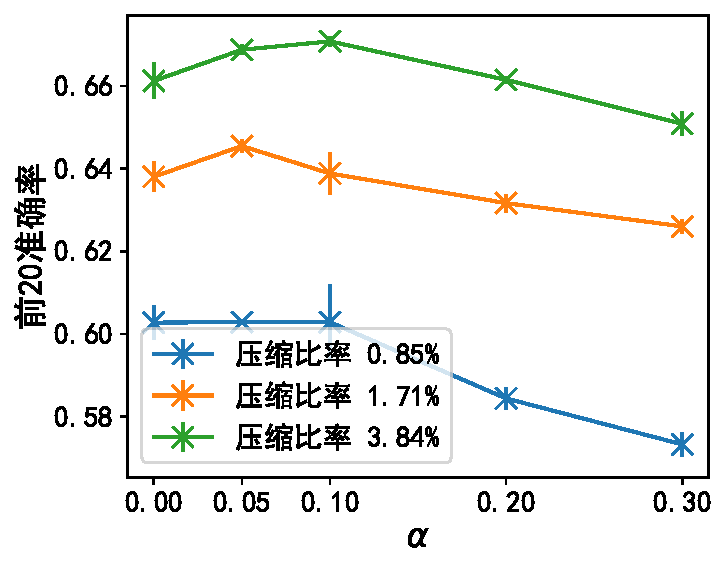
\includegraphics[width=1\linewidth]{Z_Resources/随机topk_yoochoose-alpha.pdf}
        \subcaption{YooChoose.}
        \label{fig:cifar-generror}
    \end{subfigure}
    \caption{$\alpha$与准确率的关系}
    \label{fig:randomized_topk-alpha-acc}
\end{figure}

\textbf{准确率}:
\autoref{fig:randomized_topk-alpha-acc}展示了在CIFAR-100任务中$k=3$情况下,随机参数$\alpha$与模型测试准确率的关系。
可以看出,在CIFAR-100任务中,无论怎样选取$\alpha$都可以比无压缩情况下显著提高准确率,而在YooChoose任务中,提高的幅度则相对有限。
同时,在$\alpha$ 提高到 0.1之后,准确率随着$\alpha$的进一步提高呈现出下降趋势。
%
分析表明,$\alpha \in [0.5, 1]$ 可以使得模型达到较高准确率;而过大的$\alpha$会引入过多的噪声,从而损害模型的效果。


\begin{figure}[h!]
    \centering
    \begin{subfigure}{0.45\linewidth}
        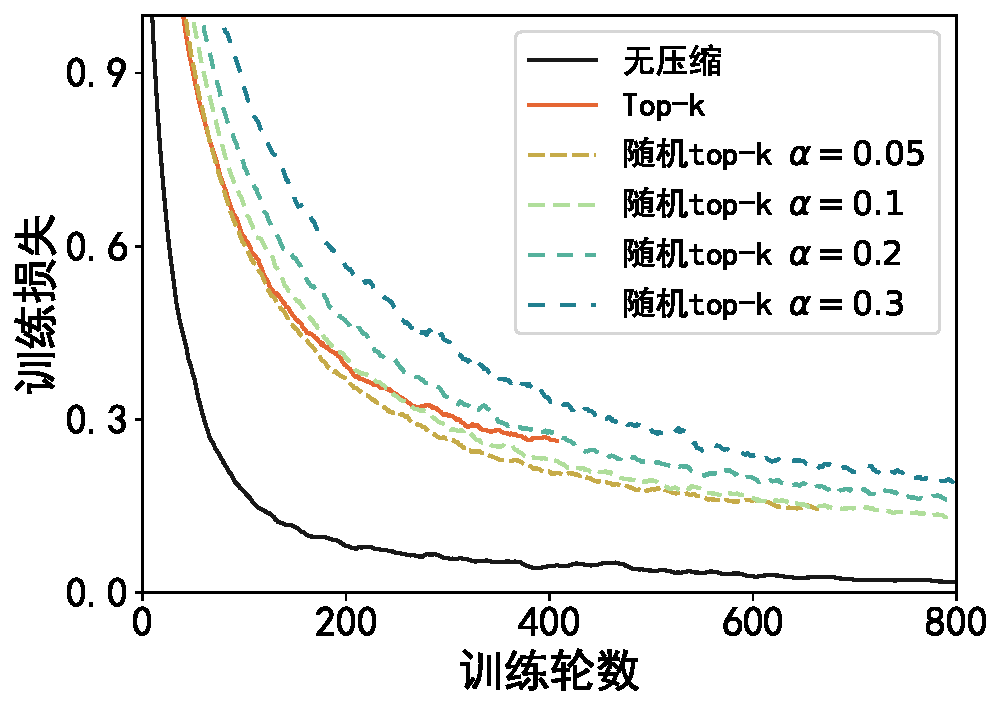
\includegraphics[width=1\linewidth]{Z_Resources/随机topk_cifar100-trainacc.pdf}
        \subcaption{训练损失.}
        \label{fig:randomized_topk-cifar-trainloss}
    \end{subfigure}
    \begin{subfigure}{0.47\linewidth}
        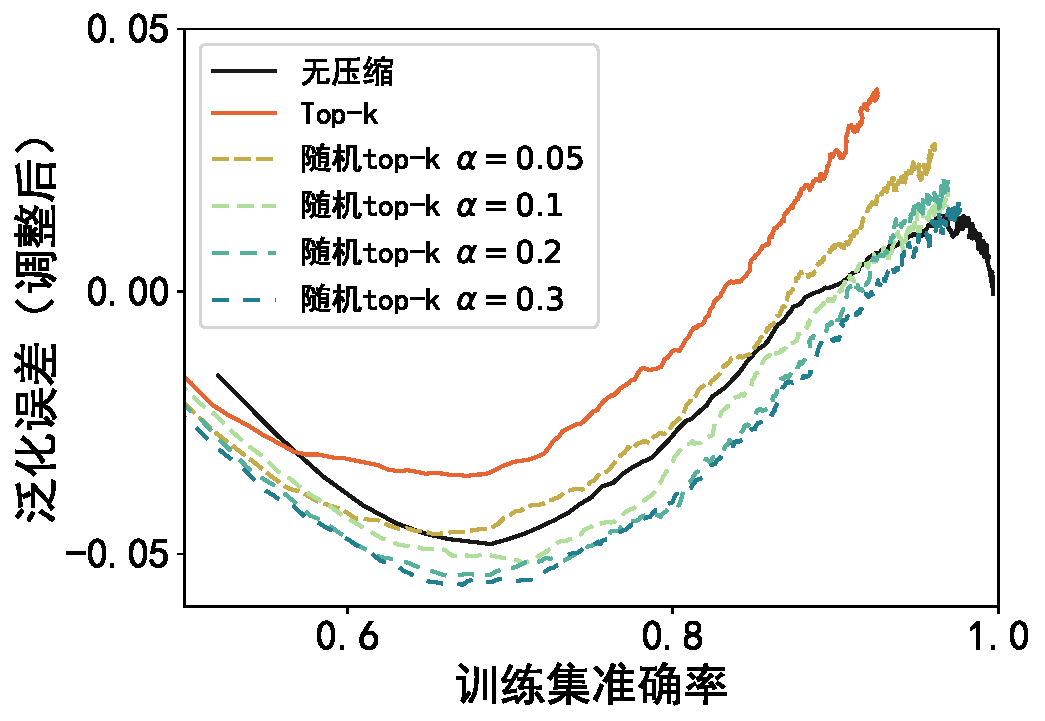
\includegraphics[width=1\linewidth]{Z_Resources/随机topk_cifar100-generror.pdf}
        \subcaption{泛化误差.}
        \label{fig:randomized_topk-cifar-generror}
    \end{subfigure}
    \caption{$\alpha$与训练损失以及泛化误差的关系}
    \label{fig:randomized_topk-alpha-loss}
\end{figure}
\textbf{收敛性和泛化误差}:
\autoref{fig:randomized_topk-alpha-loss}展示了在CIFAR-100任务中$k=3$情况下,随机参数$\alpha$与模型训练损失和泛化误差的关系。
为了更清晰呈现泛化误差的变化,我们再对泛化误差进行了调整,将\autoref{fig:randomized_topk-cifar-trainloss}调整为的Y轴调整为如下:
\begin{equation}
    y = \text{泛化误差(训练集准确率 - 测试集准确率)} - 0.5 \times \text{训练集准确率} + 0.2.
\end{equation}
%
从图中可以看出,top-$k$稀疏化在训练开始时损失下降较快,但是随着训练轮数的增长,随机top-$k$的损失下降变快,并且最终收敛的损失低于top-$k$。
另外,太大的$\alpha$也导致损失下降变慢。
%
同时,相对于无压缩的情况,top-$k$稀疏化显著增加了泛化误差。而增大$\alpha$也显著降低了泛化误差。
%
这和我们在\autoref{sec:randomized_topk:method}中对于随机top-$k$算法的收敛性和泛化性的理论分析相对应。



\begin{figure}[h!]
    \centering
    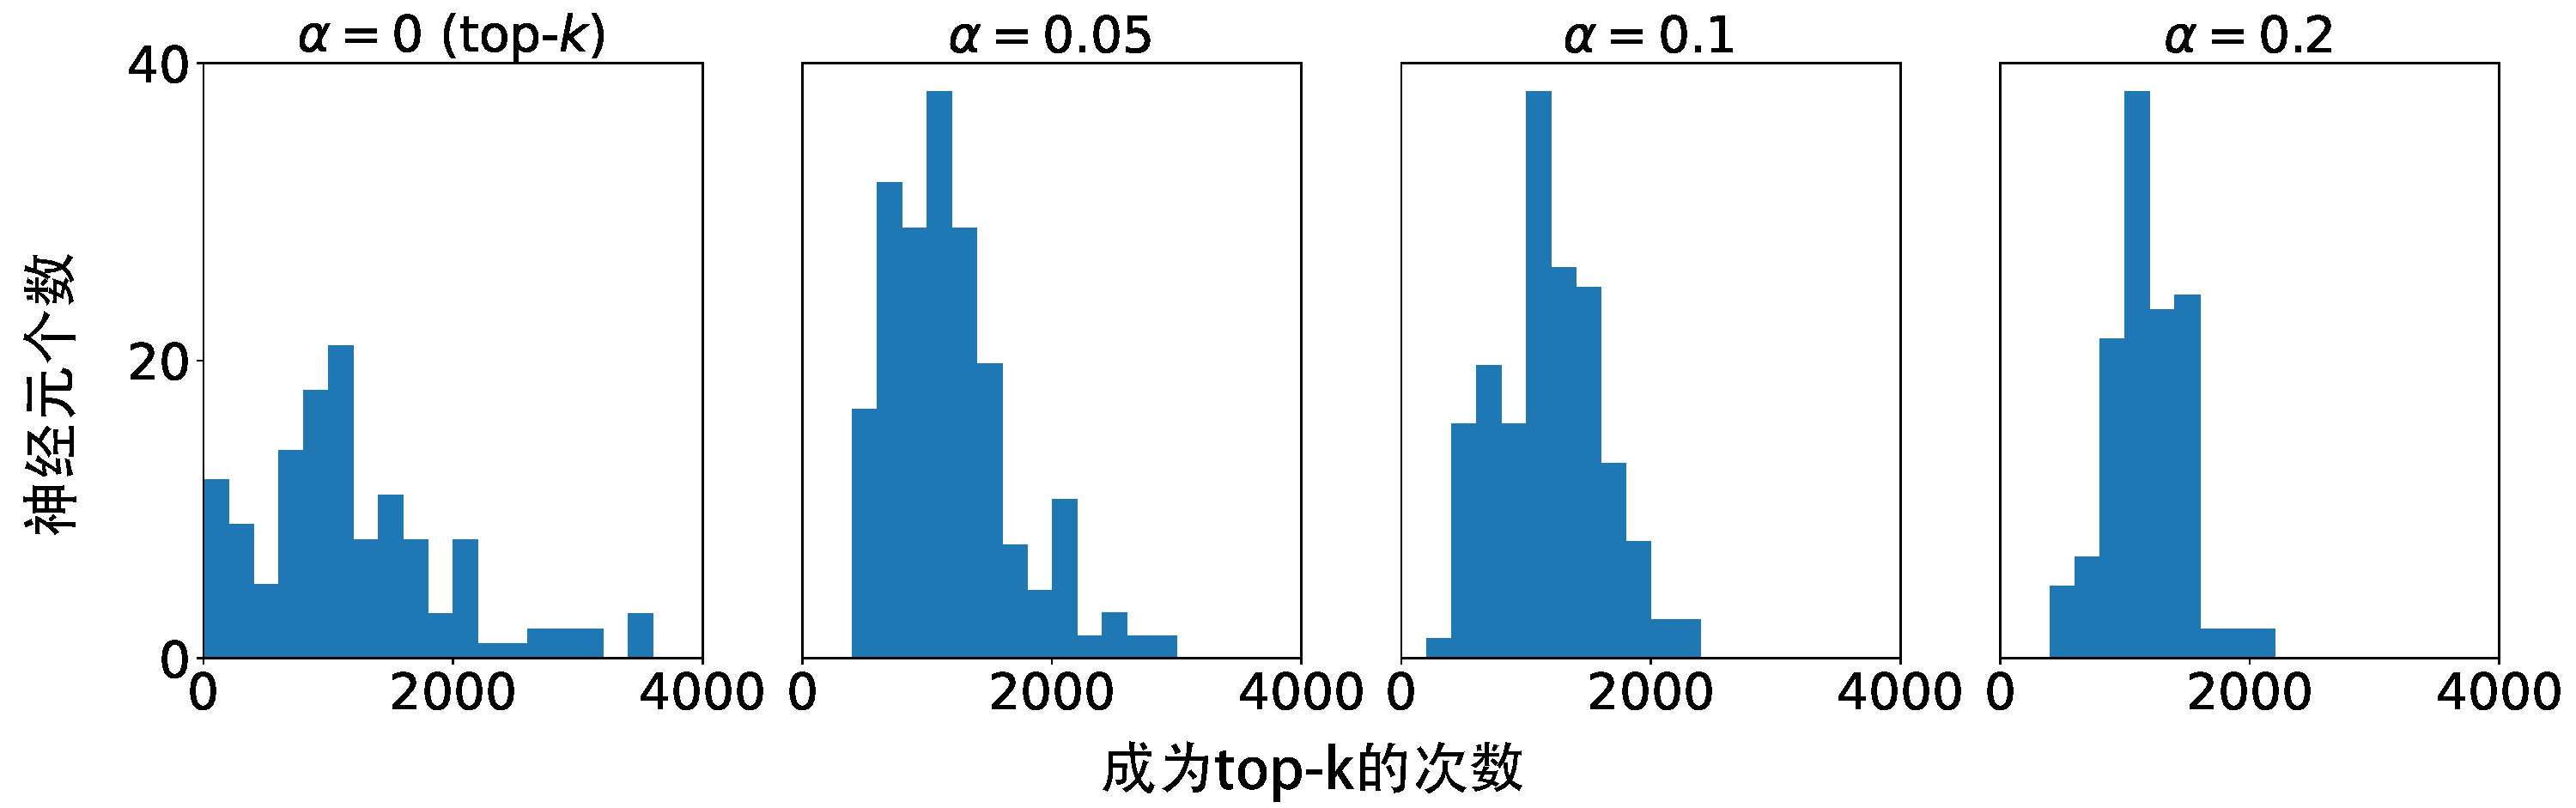
\includegraphics[width=\linewidth]{Z_Resources/随机topk_cifar100-dist-topk.pdf}
    \caption{两方拆分学习推断示意图}
    \label{fig:randomized_topk-dist}
\end{figure}

\textbf{Top-$k$神经元的分布}
\autoref{fig:randomized_topk-dist}显示了采用不同的$\alpha$训练后,在推断阶段使用测试集样本时,神经元被选为top-$k$次数的分布。具体而言,隐层的第$i$个神经元被选为top-$k$的次数按照如下公式计算:
\begin{equation}
    C_i = \sum_{j=1}^N [\text{$M_b(X_j)$的 top-$k$ 神经元包含了其第 $i$ 个神经元(是=1,否=0)}],
\end{equation}
其中,$N$表示测试集样本数,$X_j$表示第$j$个样本。
%
%
可以看出,仅使用top-$k$稀疏化时,神经元被选为top-$k$次数的分布不均匀,部分神经元几乎从未被选为top-$k$,而某些神经元则总是被选中;而使用随机top-$k$有效地解决了这一问题,top-$k$次数的分布变得均匀,说明各个神经元被选为top-$k$的概率更加均等。
%
即使是一个较小的$\alpha$(0.05),也能显著使得top-$k$次数的分布变得均匀。
%
这也说明,随机top-$k$更好地利用了表征空间,从而提高了泛化性能。
%


\begin{figure}[htbp]
    \centering
    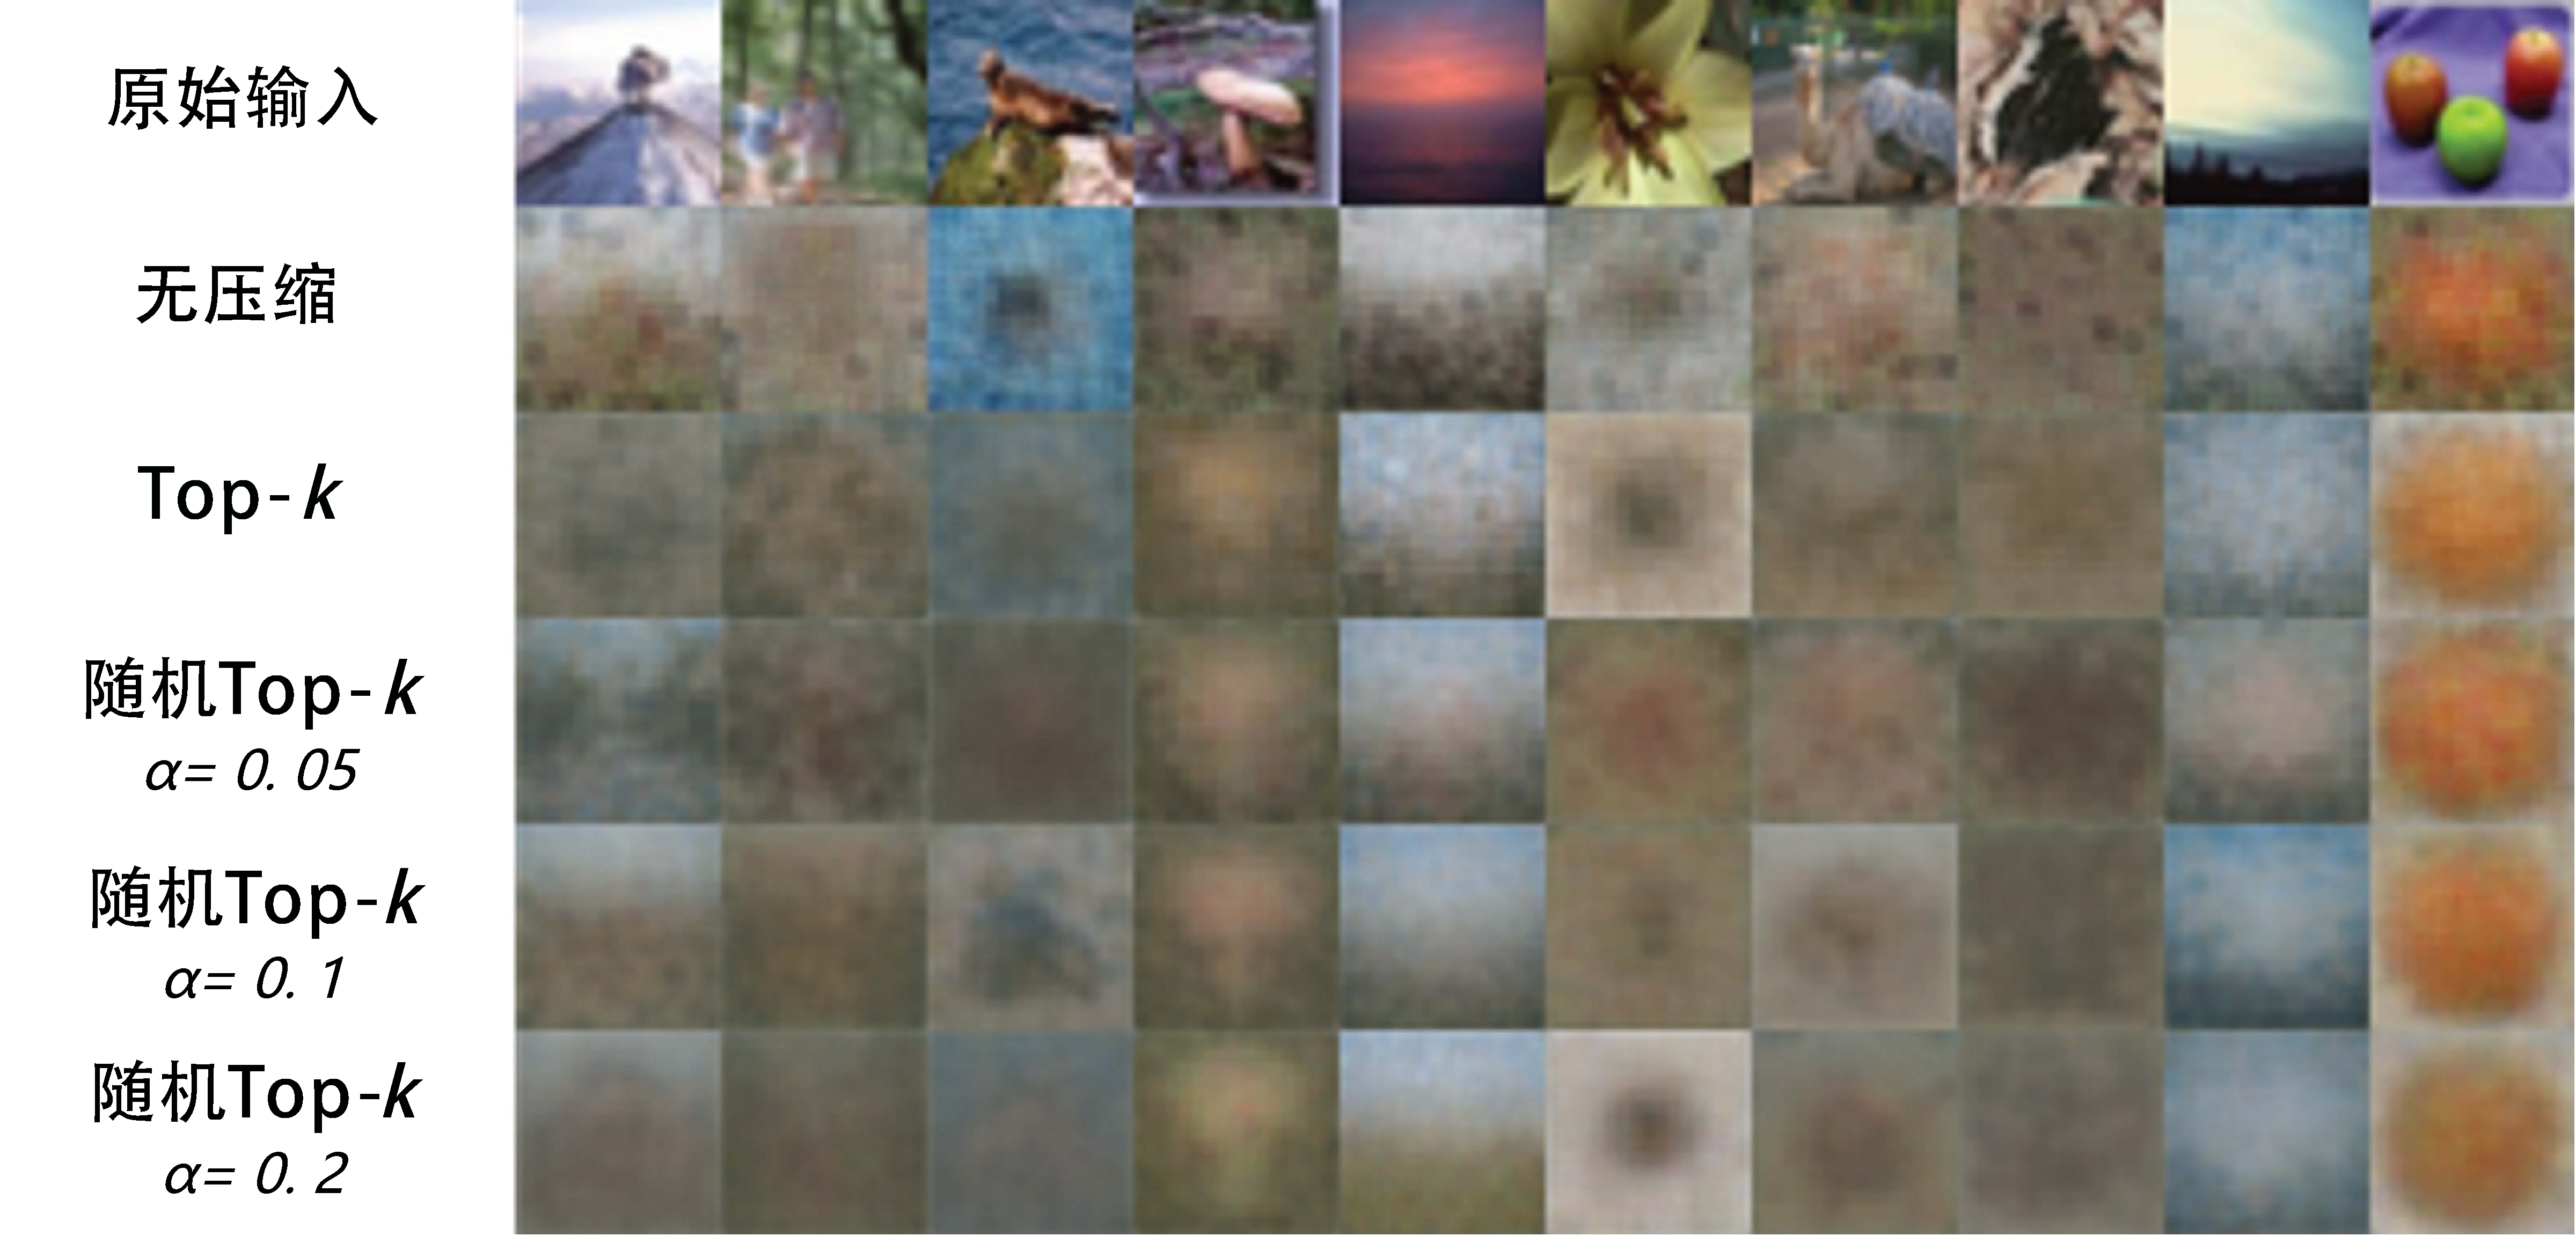
\includegraphics[width=\linewidth]{Z_Resources/随机topk_inversion-attack.pdf}
    \caption{CIFAR-100输入重建攻击效果}
    \label{fig:randomized_topk-inversion_attack}
\end{figure}

\begin{figure}[h!]
    \centering
    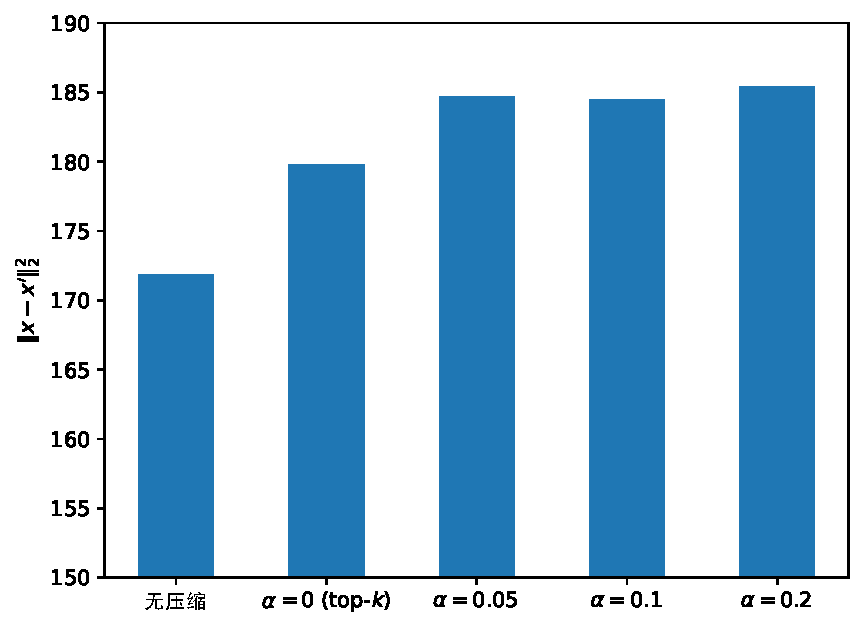
\includegraphics[width=0.58\linewidth]{Z_Resources/随机topk_attack-error.pdf}
    \caption{CIFAR-100输入重建攻击误差}
    \label{fig:randomized_topk-attack-error}
\end{figure}


\subsection{隐私分析}
为了表明随机top-$k$压缩方法对于输入数据的隐私的影响,我们在CIFAR-100数据集上进行了输入特征重建攻击的实验。
%
输入重建攻击是一种从隐层恢复出输入数据的手段,其方法是通过泄漏的数据,训练一个重构神经网络将拆分层数据逆向回原始输入特征~\cite{hezecheng_2019_model_inversion_attack,vepakomma2020nopeek}。
%
本实验中,重构神经网络的结构为(全连接,卷积,反卷积,卷积),其中全连接层将128维拆分层投影为$4 \times 16\times 16$ (4表示频道数),此后三层的输出大小分别为$16\times 16 \times  16$,$32\times 32 \times 32$,$3\times 32 \times 32$。激活函数为LeakyReLU~\cite{maas2013leaky_relu}。

\autoref{fig:randomized_topk-inversion_attack}展示了在CIFAR-100任务中$k=3$情况下,在模型推断阶段,攻击者根据拆分层表征对原始输入图片进行恢复攻击的效果。
从图中可以看出,由于拆分层被设置在最后一层线性层,因此即使是无压缩的情况下,攻击者依然难以还原图片的主要信息,只能呈现出模糊的类似于类别的“平均图”的图片。
%
而top-$k$和随机top-$k$进一步使得原始图片中的色彩信息几乎也被丢失。
%

为了更加清晰地现实随机top-$k$和其他方法的输入特征隐私保护效果,我们测量了图片恢复攻击的平方误差,即$\mathbb E\left[ \Vert \text{恢复值} - \text{原始值} \Vert_2^2 \right]$,并汇报在\autoref{fig:randomized_topk-attack-error}中。
%
从图中可以看出,top-$k$稀疏相对于原始无压缩的拆分学习显著提高了攻击者的重建损失,增强了隐私保护效果。
而随机top-$k$比top-$k$拥有更高的重建损失,说明其进一步提高了对于输入特征的隐私保护。



\section{本章小结}
本章节针对多分类拆分学习中的通信效率问题,提出了随机Top-$k$稀疏方法,并且从泛化误差、收敛性以及隐私性三个角度进行了理论和实验分析,证明了随机Top-$k$算法的优越性。
%
我们通过近似计算表征空间大小,表明了Top-$k$算法在同等压缩率下拥有更大的表征空间,从而使各个类别的决策区域更大,带来更低的泛化误差。
%
同时,通过一个二维例子说明了Top-$k$算法在收敛性上可能面临部分神经元无法被训练到的问题,而在Top-$k$中加入随机性可以有效地防止该类问题。
%
基于以上分析,我们提出随机Top-$k$算法对传统的Top-$k$进行了改进。
%
通过与Top-$k$算法、拆分层量化、L1正则化、缩小拆分层等方法对比,随机Top-$k$显示出了其在拆分学习训练与推断过程中的优越性,包含了更高的模型准确率和训练/推断速度。
%
此外,实验结果也表明稀疏化后的拆分层表征也能降低对于输入特征的隐私泄漏问题。
%
总之,随机Top-$k$算法显著提高了类别数量众多时拆分学习训练和推断过程中的通信效率,为拆分学习模型在实际应用中的部署提供了有力支持。
